\section{Model training and testing}

Starting from the features selected in the previous steps, a model prediction phase followed. This has been done, first of all, using the k-fold cross validation technique. It has been applied with a number of folders equal to 10 and repeated more than one time as suggested in \cite{traffic}. In this work the validation was repeated for a number of iterations equal to 10.

\begin{figure}[H]
\centering
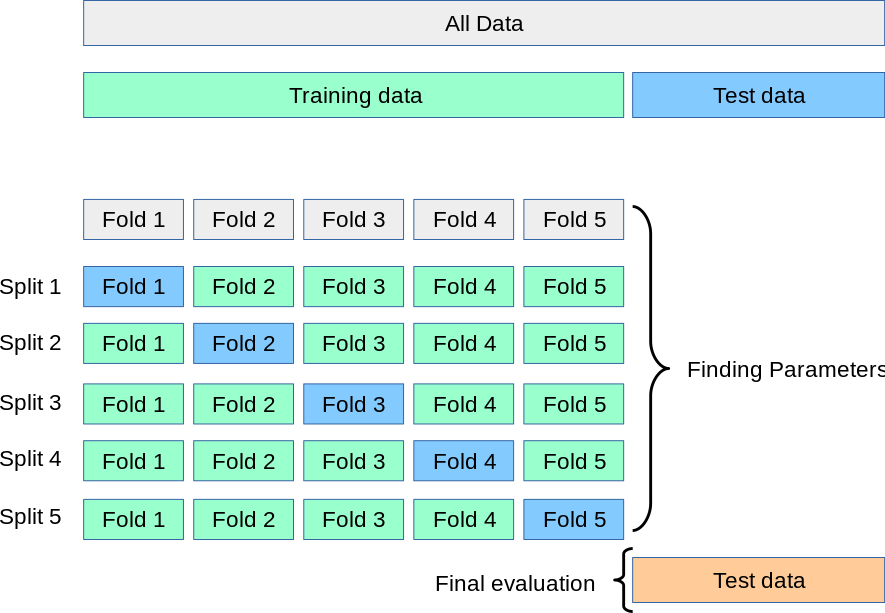
\includegraphics[width=10cm]{images/training/cross_validation.png}
\caption{Cross-validation example}
\label{cross-validation}
\end{figure}

\noindent
The output, composed by ten elements, each one representing the mean of the accuracy of one 10-fold iteration, has been used in order to perform the statistical test.

\subsection{Model selection}

Some classifiers have been discarded after comparing some parameters shown in \ref{fig:75-85}: \emph{K Nearest}, \emph{Decision Tree} and \emph{Stochastic Gradient} because of their low accuracy compared to the others and \emph{Random Forest}, \emph{Gradient Boosting}, \emph{Bagging} and \emph{Ada Boost} because of their high execution time.

\noindent
The remaining classifiers have been compared in terms of accuracy (more than 70\%), precision, recall and f1-score.

\vspace{5mm}

\setlength{\tabcolsep}{5pt}
\renewcommand\arraystretch{1.5}
\begin{table}[H]
\centering
\begin{tabular}{lc cc c cc c cc}
\hline
\multirow{2}*{Classifier} & \multirow{2}*{Accuracy (\%)} & \multicolumn{2}{c}{Precision (\%)} && \multicolumn{2}{c}{Recall (\%)} && \multicolumn{2}{c}{F1-score (\%)}\\
\cline{3-4} \cline{6-7} \cline{9-10}
\multicolumn{1}{c}{} && 0 & 1 && 0 & 1 && 0 & 1 \\
\hline
Logistic Regression & 72.52 & 71.00 & 74.28 && 76.14 & 68.90 && 73.48 & 71.49 \\
SVM                 & 71.76 & 70.63 & 73.02 && 74.49 & 69.03 && 72.51 & 70.97 \\
\hline
\end{tabular}
\caption{Report comparison \emph{Logistic Regression} and \emph{SVM}}
\label{training-LR-SVM}
\end{table}

\noindent
\emph{Logistic Regression} performs better than \emph{SVM} considering all the metrics (Table  \ref{training-LR-SVM}). 

\setlength{\tabcolsep}{5pt}
\renewcommand\arraystretch{1.5}
\begin{table}[H]
\centering
\begin{tabular}{lc cc c cc c cc}
\hline
\multirow{2}*{Classifier} & \multirow{2}*{Accuracy (\%)} & \multicolumn{2}{c}{Precision (\%)} && \multicolumn{2}{c}{Recall (\%)} && \multicolumn{2}{c}{F1-score (\%)}\\
\cline{3-4} \cline{6-7} \cline{9-10}
\multicolumn{1}{c}{} && 0 & 1 && 0 & 1 && 0 & 1 \\
\hline
ComplementNB        & 73.03 & 72.21 & 73.91 && 74.87 & 71.19 && 73.52 & 72.52 \\
MultinomialNB       & 72.39 & 71.87 & 72.95 && 73.60 & 71.19 && 72.72 & 72.06 \\
\hline
\end{tabular}
\caption{Report comparison of \emph{ComplementNB} and \emph{MultinomialNB}}
\label{training-CNB-MNB}
\end{table}

\noindent
Comparing the Naive Bayes classifiers, \emph{ComplementNB} is preferred (Table  \ref{training-CNB-MNB}).

\subsection{Paired t-test}

The paired t-test has been performed to compare the four classifiers two-by-two to establish if their performances are statistically different or not starting from a null hypothesis saying that they are the same or, in other words, that the difference in mean error rate between the two is zero. If we can reject this hypothesis, then we can conclude that the difference between the two models is statistically significant, so can be selected the model with the lower error rate (higher accuracy) \cite{book}.

The scores obtained are k=10 and the degree of freedom considered are k-1. By computing the t-statistic value and using a significance level \begin{math}sig = 0.05\end{math} and a confidence limit of \begin{math}z = 0.025\end{math} (that is half of sig) some considerations can be done comparing t with a value j obtained from the t-distribution table: if \begin{math}t > j\end{math} or \begin{math}t < -j\end{math} the null hypothesis is rejected and there is statistically significant difference between the two models, otherwise the hypothesis cannot be rejected and this means that any difference between them is attributed by chance.

\vspace{5mm}

\noindent
Figure \ref{t-test} shows the result of the paired t-test executed on the 4 different classifiers.


\begin{figure}[H]
\centering
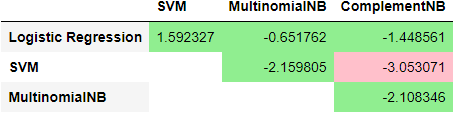
\includegraphics[width=10cm]{images/training/t_test_result.png}
\caption{Student T-test result}
\label{t-test}

\begin{figure}[H]
\end{figure}
\centering
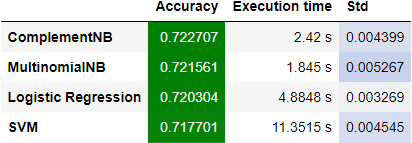
\includegraphics[width=10cm]{images/training/best_cv.png}
\caption{Performances compared}
\end{figure}

\noindent
The pink cells indicate the comparable classifiers while the green ones are related to the non-comparable ones. Reading Table \ref{t-test} row by row some considerations can be done:
\begin{itemize}
    \item The difference between \emph{SVM} and \emph{ComplementNB} is statistically significant, but \emph{SVM} has a worse accuracy with respect to \emph{ComplementNB}, so ComplementNB have been chosen;
\end{itemize}

\noindent
At the end, \emph{ComplementNB}, \emph{MultinomialNB} and \emph{Logistic Regression} models are taken into consideration and used for the test phase. 

\begin{figure}[h]
\centering
\begin{minipage}[c]{0.48\textwidth}
\centering
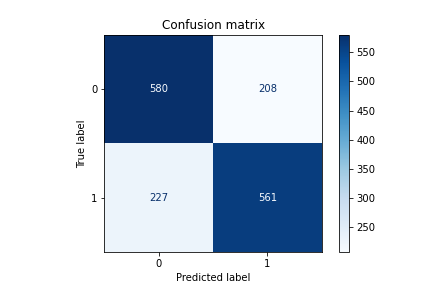
\includegraphics[width=8cm]{images/training/MultinomialNB-confusion_matrix.png}
\caption{MultinomialNB}
\end{minipage}
\begin{minipage}[c]{0.48\textwidth}
\centering
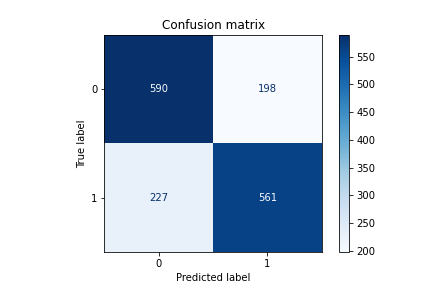
\includegraphics[width=8cm]{images/training/ComplementNB-confusion_matrix.png}
\caption{ComplementNB}
\end{minipage}
\end{figure}


\begin{figure}[H]
\centering
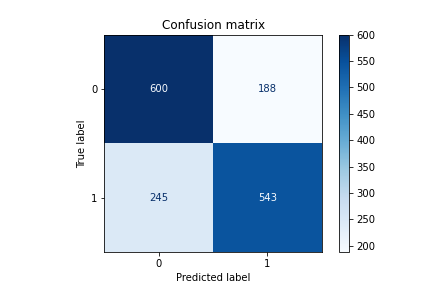
\includegraphics[width=8cm]{images/training/Logistic Regression-confusion_matrix.png}
\caption{LogisticRegression}
\end{figure}


\subsection{Model testing}

After the model building phase, the test phase has been performed. In order to test the performance of the models, 176 tweets from February were randomly and manually labeled, corresponding to a proportion 90:10 with respect to the training set. Testing the models built in the precedent phase, the results shown in Table \ref{table:test} below have been obtained. 
\vspace{5mm}
\begin{table}[H]
\centering
\setlength{\tabcolsep}{5pt}
\renewcommand\arraystretch{1.5}
\begin{tabular}{lc cc c cc c cc}
\hline
\multirow{2}*{Classifier} & \multirow{2}*{Accuracy (\%)} & \multicolumn{2}{c}{Precision (\%)} && \multicolumn{2}{c}{Recall (\%)} && \multicolumn{2}{c}{F1-score (\%)}\\
\cline{3-4} \cline{6-7} \cline{9-10}
\multicolumn{1}{c}{} && 0 & 1 && 0 & 1 && 0 & 1 \\
\hline
ComplementNB                 & 73.29 & 71.13 & 75.94 && 78.40 & 68.18 && 74.59 & 71.85 \\
Logistic Regression         & 71.59 & 68.26 & 76.38 && 80.68 & 62.50 && 73.95 & 68.75 \\
MultinomialNB                 & 73.29 & 71.13 & 75.94 && 78.40 & 68.18 && 74.59 & 71.85 \\
\hline
\end{tabular}
\caption{Report comparison of Logistic Regression and ComplementNB}
\label{table:test}
\end{table}

\noindent
As shown in Table \ref{table:test}, ComplementNB and MultinomialNB performs a little bit better than the training set instead of the Logistic Regression which performs a little worse. ComplementNB and MultinomialNB have the same performance in this phase but ComplementNB have been chosen because of its better performance in the training set phase. 